
%(BEGIN_QUESTION)
% Copyright 2012, Tony R. Kuphaldt, released under the Creative Commons Attribution License (v 1.0)
% This means you may do almost anything with this work of mine, so long as you give me proper credit

Suppose the electric motor refuses to run when the ``Run'' pushbutton switch is pressed.  A technician begins diagnosing the circuit, following the steps shown (in order):

$$\includegraphics[width=15.5cm]{i00975x01.eps}$$

\begin{itemize}
\item{} {\bf Test 1:} Measured 12 volts DC between points {\bf C} and {\bf D}, with ``Run'' switch pressed.
\vskip 25pt
\item{} {\bf Test 2:} Measured 0 volts DC between points {\bf A} and {\bf C}, with ``Run'' switch unpressed.
\vskip 25pt
\item{} {\bf Test 3:} Measured 12 volts DC between points {\bf A} and {\bf B}, with ``Run'' switch pressed.
\vskip 25pt
\item{} {\bf Test 4:} Measured 12 volts DC between points {\bf E} and {\bf F}, with ``Run'' switch pressed.
\vskip 25pt
\item{} {\bf Test 5:} Measured infinite ohms between points {\bf E} and {\bf F}, with ``Run'' switch unpressed. 
\vskip 25pt
\medskip

Identify any useful information about the nature or location of the fault derived from the results of each test, in order of the tests performed.  If the test is not useful (i.e. provides no new information), mark it as such.  Assuming there is only one fault in the circuit, identify the location and nature of the fault as precisely as you can from the test results shown above.

\underbar{file i00975}
%(END_QUESTION)





%(BEGIN_ANSWER)

{\bf The fault is an ``open,'' between points E and F.}

%(END_ANSWER)





%(BEGIN_NOTES)

\begin{itemize}
\item{} {\bf Test 1:} Measured 12 volts DC between points {\bf C} and {\bf D}, with ``Run'' switch pressed.  {\it Proves that the problem is to the right of these test points (toward the motor).  The 12 VDC source is good, and the ``Run'' switch is not faulted open.  It also proves that the fault is not a short, but must be an open.}
\vskip 5pt
\item{} {\bf Test 2:} Measured 0 volts DC between points {\bf A} and {\bf C}, with ``Run'' switch unpressed.  {\it This isn't a stictly necessary test, as we already know the fault is an open somewhere in the C-E-F-D pathway.  However, it certainly does confirm the diagnosis of an ``open'' (versus ``shorted'') fault.}
\vskip 5pt
\item{} {\bf Test 3:} Measured 12 volts DC between points {\bf A} and {\bf B}, with ``Run'' switch pressed.  {\it This is an unnecessary test, as we already know the source is not dead from Test 1.}
\vskip 5pt
\item{} {\bf Test 4:} Measured 12 volts DC between points {\bf E} and {\bf F}, with ``Run'' switch pressed.  {\it Proves the problem is an ``open'' fault between these test points, most likely inside the motor.}
\vskip 5pt
\item{} {\bf Test 5:} Measured infinite ohms between points {\bf E} and {\bf F}, with ``Run'' switch unpressed.  {\it This test is not really necessary, as we already know there's an ``open'' fault between points E and F.}
\end{itemize}






\vskip 20pt \vbox{\hrule \hbox{\strut \vrule{} {\bf Virtual Troubleshooting} \vrule} \hrule}

This question is a good candidate for a ``Virtual Troubleshooting'' exercise.  Presenting the diagram to students, you first imagine in your own mind a particular fault in the system.  Then, you present one or more symptoms of that fault (something noticeable by an operator or other user of the system).  Students then propose various diagnostic tests to perform on this system to identify the nature and location of the fault, as though they were technicians trying to troubleshoot the problem.  Your job is to tell them what the result(s) would be for each of the proposed diagnostic tests, documenting those results where all the students can see.

During and after the exercise, it is good to ask students follow-up questions such as:

\begin{itemize}
\item{} What does the result of the last diagnostic test tell you about the fault?
\item{} Suppose the results of the last diagnostic test were different.  What then would that result tell you about the fault?
\item{} Is the last diagnostic test the best one we could do?
\item{} What would be the ideal order of tests, to diagnose the problem in as few steps as possible?
\end{itemize}


%INDEX% Troubleshooting review: electric circuit diagnostic test rationale

%(END_NOTES)


